% Template for Cogsci submission with R Markdown

% Stuff changed from original Markdown PLOS Template
\documentclass[10pt, letterpaper]{article}

\usepackage{cogsci}
\usepackage{pslatex}
\usepackage{float}

% amsmath package, useful for mathematical formulas
\usepackage{amsmath}

% amssymb package, useful for mathematical symbols
\usepackage{amssymb}

% hyperref package, useful for hyperlinks
\usepackage{hyperref}

% graphicx package, useful for including eps and pdf graphics
% include graphics with the command \includegraphics
\usepackage{graphicx}

% Sweave(-like)
\usepackage{fancyvrb}
\DefineVerbatimEnvironment{Sinput}{Verbatim}{fontshape=sl}
\DefineVerbatimEnvironment{Soutput}{Verbatim}{}
\DefineVerbatimEnvironment{Scode}{Verbatim}{fontshape=sl}
\newenvironment{Schunk}{}{}
\DefineVerbatimEnvironment{Code}{Verbatim}{}
\DefineVerbatimEnvironment{CodeInput}{Verbatim}{fontshape=sl}
\DefineVerbatimEnvironment{CodeOutput}{Verbatim}{}
\newenvironment{CodeChunk}{}{}

% cite package, to clean up citations in the main text. Do not remove.
\usepackage{cite}

\usepackage{color}

% Use doublespacing - comment out for single spacing
%\usepackage{setspace}
%\doublespacing


% % Text layout
% \topmargin 0.0cm
% \oddsidemargin 0.5cm
% \evensidemargin 0.5cm
% \textwidth 16cm
% \textheight 21cm

\title{A speed-accuracy trade-off in children's processing of scalar
implicatures}


\author{{\large \bf Rose M. Schneider} \\ \texttt{rschneid@stanford.edu} \\ Department of Psychology \\ Stanford University \And {\large \bf Michael C. Frank} \\ \texttt{mcfrank@stanford.edu} \\ Department of Psychology \\ Stanford University}

\begin{document}

\maketitle

\begin{abstract}
Scalar implicatures---inferences from a weak description (``I ate some
of the cookies'') that a stronger alternative is not true (``I didn't
eat all'')---are paradigm cases of pragmatic inference. Children's
trouble with scalar implicatures is thus an important puzzle for
theories of pragmatic development, given their communicative competence
in other domains. Previous research has suggested that access to
alternatives might be key. Here, we explore children's reaction times in
a new paradigm for measuring scalar implicature processing. Alongside
failures on scalar implicatures with ``some,'' we replicate previous
reports of failures with ``none,'' and find evidence of a speed-accuracy
trade-off for both quantifiers. Motivated by these findings, we explore
the relationship between accuracy and reaction time with a Drift
Diffusion Model. We find evidence consistent with the hypothesis that
preschoolers lack access to relevant alternatives for scalar implicature
computation, although this set of alternatives may be broader than
previously assumed.

\textbf{Keywords:}
Pragmatics; development; scalar implicature; diffusion models.
\end{abstract}

\section{Introduction}\label{introduction}

Language comprehension in context is an inferential process. Listeners
are not limited to interpreting the literal meaning of speakers'
utterances; they can also reason about what the speaker intended, based
on alternative utterances. In the case of \emph{pragmatic implicatures}
(Grice, 1975), a speaker employs a weaker literal description to imply
that a stronger alternative is true. Adult listeners tend to infer from
the statement ``I ate \emph{some} of the cookies'' that some, but not
all, of the cookies remain. This \emph{scalar implicature} (SI) relies
heavily on a knowledge of the relevant lexical alternatives in the
quantifier scale \(<\)\emph{some}, \emph{all}\(>\). On standard
theories, a listener must be able to contrast ``some'' with the stronger
descriptor ``all'' to compute the implicature (Grice, 1975; Levinson,
2000).

SIs are challenging for children until surprisingly late in development
(Noveck, 2001). For example, when judging a scene in which three of
three horses have jumped over a fence, five-year-olds are likely to
endorse the statement ``some of the horses jumped over the fence'' as
felicitous, despite the availability of a more informative alternative
(``all''; Papafragou \& Musolino, 2003). Children do seem to have some
knowledge of these scalar terms, however; for example, they
differntially reward speakers based on the informativeness of their
scalar descriptions (Katsos \& Bishop, 2011). Given this early
sensitivity, why do children still struggle to compute scalar
implicatures until fairly late in development?

One possible cause of children's failures is that they may not have
access to the relevant lexical alternatives (Barner \& Bachrach, 2010).
This idea, which we will refer to as the \emph{Alternatives Hypothesis},
predicts that if children cannot quickly and reliably bring to mind the
relevant alternative quantifiers (e.g., ``all'' in a situation where
they hear ``some'') they will be unable to make the implicature
computation. The alternatives hypothesis makes a number of predictions
about children's abilities in reasoning about quantifiers, some of which
have been confirmed empirically. For example, consistent with the idea
of inaccessible alternatives, Barner, Brooks, \& Bale (2011) showed that
four-year-olds could not compute the quantifier expression ``only some''
(which should force alternatives to be negated semantically, rather than
pragmatically). In light of this hypothesis, what are the proper
alternatives for SIs?

With respect to these alternatives, empirical evidence has been changing
rapidly. Although the conventional view on SI is that the primary
inferential alternative is ``all,'' a new body of evidence suggests that
more alternatives may be necessary. For example, Degen \& Tanenhaus
(2015) found that set size can change the felicity of quantifier SIs for
adults: ``some'' is more felicitous when participants could not say
``one'' or ``two.'' In a computational reanalysis of Degen \& Tanenhaus
(2015) and other data, Franke (2014) showed that a high weight on the
alternative ``none'' was critical for fitting these data. And in a
recent study with children, Skordos \& Papafragou (in press) found that
exposing children to either ``all'' \emph{or} ``none'' facilitated their
computation of subsequent SIs. Taken together, these data suggest that
the availability of alternatives---in particular ``none''---does affect
scalar implicature processing.

This relationship to ``none'' is unexpected on classic Gricean theories
(Grice, 1975; Horn, 1972), where the only alternatives should be those
logically entailed by the original message (i.e. ``all''). But it
\emph{is} in fact predicted by recent probabilistic models of
implicature. Under these models, all the relevant alternatives compete
with one another (Franke, 2014; Goodman \& Stuhlmuller, 2013). On the
other hand, all of the evidence cited above for the claim of ``none'' as
an alternative is relatively indirect, and such a substantial revision
to theory requires further evidence.

\begin{CodeChunk}
\begin{figure}[b]

{\centering 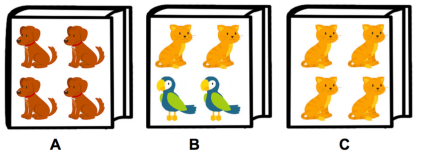
\includegraphics{figs/image-1} 

}

\caption[Example trial stimuli used in Horowitz and Frank (2015)]{Example trial stimuli used in Horowitz and Frank (2015).}\label{fig:image}
\end{figure}
\end{CodeChunk}

One other recent developmental study further supports the importance of
``none'' in SIs and provides the starting point for our current
experiment. Horowitz \& Frank (2015) designed a referent selection
paradigm that could be used across a broad age range (3--5 years) to
explore both scalar and ad-hoc (context-dependent) implicatures. In this
task, children saw three book covers, each featuring four familiar
objects (Figure \ref{fig:image}). On target trials, the experimenter
described a book using a semantically ambiguous description (e.g., ``On
the cover of my book, some of the pictures are cats'' {[}scalar{]} or
``On the cover of my book are cats'' {[}ad hoc{]}). Children succeeded
on ad-hoc trials but largely failed to make SIs, suggesting they had the
pragmatic competence necessary to compute the implicature, but failed to
do so for scalar descriptors.

Interestingly, in Horowitz \& Frank (2015), the same children who failed
on SI also failed on unambiguous ``none'' control trials (e.g., ``On the
cover of my book, \emph{none} of the pictures are cats''``)---and in
several samples, performance was highly correlated between''none" and
``some'' trials. This result would be predicted if ``none'' were in fact
an inferential alternative to ``some.'' If children were not computing
its semantics appropriately in an online fashion, they would fail in the
``some'' SI computation as well, leading to a correlation.

One further prediction of the alternatives hypothesis relates to
processing time. Perhaps children who have a fully-established
quantifier scale---and hence can make correct SIs---take additional time
in using this information, due to competition between alternatives.
Congruent with this prediction, our intuition in Horowitz \& Frank
(2015) and Horowitz, Schneider, \& Frank (in prep.) was that when
children made correct SIs they appeared to be taking longer than when
they failed. Motivated by this observation, we adapted our SI task for
the iPad to collect detailed and accurate developmental reaction time
data. Although reaction time measures have been commonplace in studies
of adults' SI processing, they have been almost entirely absent in the
developmental literature (with the exception of Huang \& Snedeker, 2009,
whose data showed little evidence of SI computation).

Thus, in our current study, we explore children's behavioral response
latencies in an iPad adaptation of the Horowitz \& Frank (2015) scalar
implicature task. Due to the large sample size and number of trials per
participant in Horowitz \& Frank (2015) and Horowitz et al. (in prep.),
manually coding video of previous trials was prohibitive. In our
analyses, we examine overall accuracy and patterns of performance, as in
Horowitz \& Frank (2015), and find that children not only struggle in
making a scalar implicature, but replicate the finding that they have
difficulty with ``none'' until fairly late in development. Congruent
with our predictions, in examining reaction time patterns across all
quantifier types, we find evidence of a speed-accuracy trade-off for
both quantifiers, such that children who succeed exhibit longer response
latencies. Finally, we use a Drift Diffusion Model (Ratcliff, 1978;
Ratcliff \& Rouder, 1998) to explore the source of this increased
reaction time. Overall, our findings are consistent with a version of
the Alternatives Hypothesis under which ``none'' is an important
inferential alternative in SI and its availability causes slower
processing times but correct SIs.

\section{Method}\label{method}

In this study, we adapted the scalar implicature paradigm developed by
Horowitz \& Frank (2015) for the iPad. In addition to capturing detailed
reaction time data, this version included more trials, and standardized
prosody across all trials, as well as a completely randomized
design.\footnote{The full experiment can be viewed online at \texttt{https://rosemschneider.github.io/tablet\_exp/si\_tablet.html} and all of our data, processing, experimental stimuli, and analysis code can be viewed in the version control repository for this paper at: \texttt{https://github.com/rosemschneider/SI\_tablet}.}

\subsection{Participants}\label{participants}

\begin{table}[t]
\centering
\begin{tabular}{c c c c c } 
 \hline
 Age group & N & Mean & Median & SD \\
 \hline
 3--3.5 years & 24 & 3.27 & 3.27 & 0.15\\
 3.5--4 years & 35 & 3.78 & 3.73 & 0.15 \\ 
 4--4.5 years & 25 & 4.28 & 4.28 & 0.15\\
 4.5--5 years & 30 & 4.76 & 4.76 & 0.15 \\
 5--6.5 years & 24 & 5.55 & 5.56 & 0.36 \\
 \hline
\end{tabular}
\caption{Age information for all participants.}
\label{tab:age}
\end{table}

Table \ref{tab:age} shows the breakdown of age information for all
participants. Included in analyses are 138 children out of a planned
sample of 120 participants, recruited from both a local daycare and a
local children's museum. We ran 20 additional children, who were
excluded from analysis based on planned exclusion criteria of low
English language exposure (\(\leq 75\%\)) or \(<50\%\) of trials
completed. Included in our sample were 79 females and 59
males.\footnote{Based on Horowitz \& Frank (2015), we initially planned
  to collect data from children 3--5 years. After collecting data from
  57 participants, however, we observed significantly lower performance
  on implicature trials across all age groups, indicating that the iPad
  adaptation of the scalar implicature task was slightly more
  challenging for all children, and included an older age group of 24
  5--6.5-year-olds.}

\subsection{Stimuli and design}\label{stimuli-and-design}

The general format of the task was identical to Horowitz \& Frank
(2015), with the exception of added items for additional trials. The
study was programmed in HTML, CSS, and JavaScript, and displayed to
children on a full-sized iPad. Each trial displayed three book covers,
each containing a set of four familiar objects (Figure \ref{fig:image}).
Each session involved 30 trials, with 10 trials per quantifier-type
(``all'', ``some'', and ``none''). Each audio clip used the same three
initial sentence frames (e.g., ``On the cover of my book, \emph{some} of
the pictures\ldots{}'') so that prosody was emphasized equally across
all trials. The average length of each audio clip (including target item
phrase, e.g., ``\ldots{}are cats'') was approximately 6s. In our
randomization, quantifier triad order, items (within category), target
item, and quantifier were randomized for all participants. In all, there
were 270 different target items and audio clips.

\subsection{Procedure}\label{procedure}

Sessions took place individually in a small testing room away from the
museum floor or the classroom of the daycare. To familiarize children
with the iPad, each session began with a ``dot game,'' which required
them to press dots on the screen as fast as possible. After the dot
game, the experimenter introduced them to ``Hannah,'' a cartoon
character who wanted to play a guessing game with her books. The
experimenter explained that Hannah would show the child three books, and
would give one hint about which book she had in mind, so they had to
listen carefully. Children then saw a practice trial with an unambiguous
noun referent.

Each trial allowed 2.5s for children to visually inspect the three book
covers before the experiment played the trial prompt (e.g., ``On the
cover of my book, \emph{none} of the pictures are cats.''). Reaction
times were measured from the onset of the target word. Children could
only make one selection. If a child was not paying attention, or if she
did not hear Hannah's prompt, the experimenter repeated it, matching the
original prosody. Once children made their selection, a green box
appeared around the chosen book. The experiment was self-paced, and
children initiated each trial by pressing a button that appeared after
they had made their selection in the previous trial.

\begin{CodeChunk}
\begin{figure}[t]
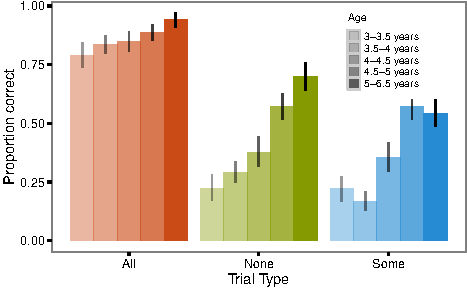
\includegraphics{figs/overall_acc-1} \caption[Children's overall accuracy for each quantifier type]{Children's overall accuracy for each quantifier type. Bars show mean performance for each age group. Error bars are 95 percent confidence intervals computed by non-parametric bootstrap.}\label{fig:overall_acc}
\end{figure}
\end{CodeChunk}

\section{Results}\label{results}

For trials where the child had missed the prompt or was not paying
attention, we excluded reaction times (RTs) longer than 15s. After this
initial cut, we excluded RTs outside three standard deviations of the
log of mean reaction time. This cleaning process resulted in RT data
loss for 85 trials (2.09\%).

\subsection{Accuracy}\label{accuracy}

Figure \ref{fig:overall_acc} shows children's mean performance for each
trial type, split by age group. For each age group, we saw significantly
lower accuracy for the quantifiers ``some'' and ``none'' in comparison
to ``all'' (all \(p\)s \(< .01\) in two-sample t-tests for each age
group). These results generally replicate our previous findings using
this paradigm (Horowitz \& Frank, 2015), but one difference from the
previous results was in implicature trials. Children aged 3--5 years
performed significantly lower on ``some'' (implicature) trials in this
task in comparison to Horowitz et al. (in prep.) (\(p < .01\) for all
tests). Thus, while the iPad adaptation was generally successful,
implicatures were more difficult, perhaps because of the non-social
nature of the iPad interaction or the recorded audio stimuli.

\begin{CodeChunk}
\begin{figure}[t]
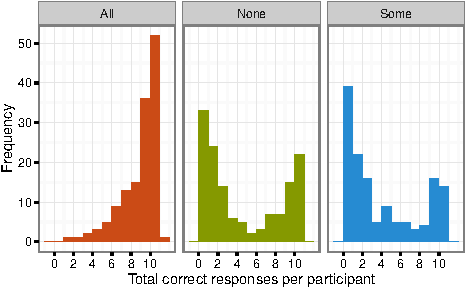
\includegraphics{figs/diptest-1} \caption[Frequency histogram of participant totals for each trial type, across all participants]{Frequency histogram of participant totals for each trial type, across all participants.}\label{fig:diptest}
\end{figure}
\end{CodeChunk}

\begin{CodeChunk}
\begin{figure*}[t]

{\centering 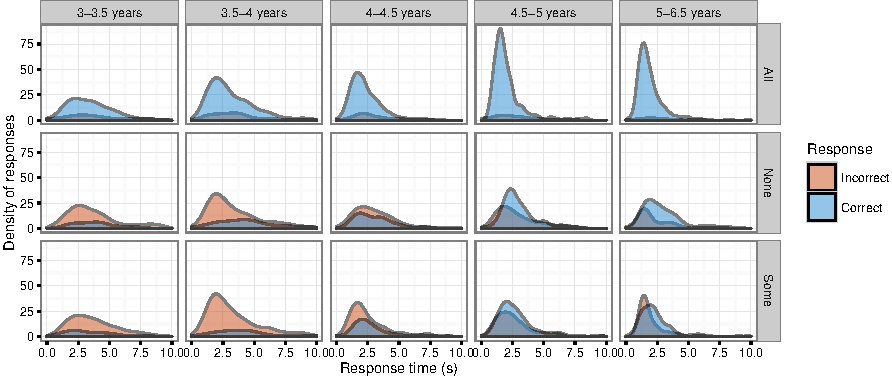
\includegraphics{figs/dense-1} 

}

\caption[Density plots of reaction times for correct and incorrect responses on each trial type, split by age]{Density plots of reaction times for correct and incorrect responses on each trial type, split by age.}\label{fig:dense}
\end{figure*}
\end{CodeChunk}

We next fit a logistic mixed effects model predicting correct response
as an interaction of age and trial type, with random effects of trial
type and
participant.\footnote{All mixed effects models were fit in \texttt{R} using the \texttt{lme4} package. The model specification was: \texttt{correct $\sim$ age * trial type + (trial type | subject id)}.}
Performance was significantly lower on ``some'' (\(\beta = -6.72\),
\(p < .0001\)) and ``none'' trials (\(\beta = -9.44\), \(p < .0001\)).
There was also a significant interaction between age and trial type on
``none'' trials (\(\beta\) = 1.52, \(p\) = .0005), indicating that
children's performance with this difficult quantifier increased with
age. This model also showed that children's performance showed a trend
towards significance for ``some'' trials (\(\beta\) = 0.76, \(p\) =
.051).

Figure \ref{fig:diptest} shows distributions of correct responses for
all trial types. Performance on ``some'' and ``none'' trials was bimodal
(Hartigan's \(D\) = 0.08, \(p\) \textless{} .0001) and ``none'' trials
(\(D\) = 0.11, \(p\) \textless{} .0001). While children's average
accuracy was low for these quantifiers, there were some children who
were correct on the majority of these trials (``Some'': N = 30;
``None'': N = 37) and the others were typically incorrect on the
majority of trials. Children did not appear to be responding randomly.
As in previous work, we found a strong correlation between children's
accuracy on ``some'' and ``none'' trials (\(r\) = 0.49, \(p\)
\textless{} .0001). Children also exhibited some interesting
systematicity in their errors: on incorrect ``some'' trials they
overwhelmingly chose ``all,'' while on ``none'' trials they also chose
``some'' at about half the rate of ``all.''

\subsection{Reaction time}\label{reaction-time}

We fit a linear mixed effects model predicting log RT on correct trials
as a function of log trial number, the interaction of age and trial
type, and random effects of trial type by subject.\footnote{Model
  specification:
  \texttt{log(reaction time) $\sim$ log(trial number) + age * trial type + (trial type | subject id)}.
  Age was centered for ease of interpretation of coefficients, and we
  calculated \emph{p} values via the \(t=z\) approximation.} Reaction
times were longer on ``none'' (\(\beta = 0.38\), \(p\) \textless{}
.0001) and ``some'' trials (\(\beta = 0.22\), \(p\) \textless{} .0001),
and reaction times decreased with age (\(\beta = -0.29\), \(p\)
\textless{} .0001). There were no significant interactions between age
and trial type. The model also showed a main effect of trial number,
with reaction times decreasing over the course of the study (\(\beta\) =
-0.1, \(p\) \textless{} .0001).

Examination of the pattern in Figure \ref{fig:dense} suggests that
accuracy and reaction time may interact, however. In particular, while
correct responses on ``all'' trials appear to be faster than the (few)
incorrect responses, the opposite is true for ``none'' and ``some''
trials: Errors have faster RTs, potentially indicating a speed-accuracy
trade-off. To test for this effect, we fit another mixed effects model,
this time including accuracy and its interactions with age and trial
type as predictors. This model revealed that correct trials overall had
faster RTs (\(\beta = -0.16\), \(p = .0002\)), but that this accuracy
term interacted negatively with trial type such that both ``none'' and
``some'' trials had slower RTs for correct trials (\(\beta = 0.34\),
\(p < .0001\); \(\beta = 0.27\), \(p < .0001\)). There were no three-way
interactions of trial-type and age. This model thus provides evidence of
a speed-accuracy trade-off for ``some'' and ``none'' trials.

\subsection{Drift diffusion models}\label{drift-diffusion-models}

\begin{CodeChunk}
\begin{figure*}[t]

{\centering 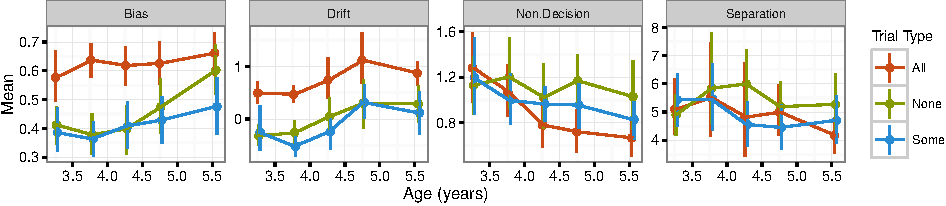
\includegraphics{figs/devo_param_plot-1} 

}

\caption[Parameter estimates for drift diffusion model, split by age and trial type]{Parameter estimates for drift diffusion model, split by age and trial type. Error bars are 95 percent confidence intervals computed by nonparametric bootstrap.}\label{fig:devo_param_plot}
\end{figure*}
\end{CodeChunk}

Motivated by the evidence of a speed-accuracy trade-off we observed, we
further explored the interaction between reaction time and accuracy in
more depth using drift diffusion modeling (DDM). DDM can be used in
behavioral tasks to provide a more detailed view of the relationship
between accuracy and reaction time (Ratcliff \& Rouder, 1998). In DDM, a
behavioral response (a correct or incorrect choice) is the result of
noisy data accumulation through a diffusion process. Responses have
\emph{separation boundaries} that are dependent on the amount of
information needed to initiate a response, and \emph{drift rate}
formalizes the rate of data accumulation. \emph{Nondecision} is the
amount of time between stimuli offset (i.e., the audio prompt), and
initiating the diffusion process. Finally, different responses may have
a \emph{bias}, or different starting point in the diffusion process,
dependent on the stimuli. Thus, a DDM can reveal more differences in the
SI decision-making process, and provide some clues about the causes
underlying the observed speed-accuracy trade-off.

\subsubsection{Developmental analyses}\label{developmental-analyses}

Although DDMs are traditionally fit to data from two-alternative
forced-choice tasks, here we estimate the drift process between a
correct and incorrect choice, with two options in each trial being
``incorrect,'' and only one being consistent with the target noun and
quantifier. We estimated parameters for each subject for each trial type
using the \texttt{RWiener} package. We then aggregated across subjects
to obtain means and confidence intervals for each age group. Figure
\ref{fig:devo_param_plot} shows the parameter estimates for each age
group, split by trial type. To fit the model, we excluded 85 trials with
outlier RTs.

For each parameter estimate, we ran a mixed effects model, predicting
parameter value as an interaction of age and trial
type.\footnote{The specifications for all parameter models are as follows: \texttt{Parameter Value $\sim$ age * trial type + (1 | subject ID)}}
For boundary separation, there was no significant effect of trial type,
indicating that roughly the same amount of information needed to be
accumulated to make a decision in each trial type. This should be
expected, given our experimental design. For non-decision time, we found
a significant main effect of age (\(\beta\) = -0.28, \(p\) \textless{}
.00001), as well as a interaction between age and ``none'' trials
(\(\beta\) = 0.24, \(p\) = .01). As expected in drift rate, there was a
negative main effect of trial type (``None'': \(\beta\) = -1.3, \(p\) =
.0185; ``Some'': \(\beta\) = -1.18, \(p\) = .03). Interestingly, for
bias there was a significant negative effect of ``none'' trials
(\(\beta\) = -0.5, \(p\) = .0005), and ``some'' trials showed a trend
towards significance (\(\beta\) = -0.28, \(p\) = .0503), as well as a
significant interaction between age and ``none'' trials (\(\beta\) =
0.07, \(p\) = .023).

In sum, the parameter estimates from our DDM align with the analyses
presented above: Older children, who are more familiar with the
quantifier scale, are more likely to respond correctly in our scalar
implicature task, while younger children's failures appear to be due to
a low rate of data accumulation and a high separation boundary.

\subsubsection{Exploratory analyses}\label{exploratory-analyses}

In addition to examining effects of age on the diffusion process, we
conducted an exploratory analysis, examining differences in the
decision-making process for children who consistently made SIs compared
with those who did not. We split children into two groups by accuracy on
scalar implicature trials, and then estimated parameters by accuracy
group. High accuracy was defined as an average of 75\% or higher
performance on scalar implicature trials. Figure \ref{fig:param_plot}
shows parameter estimates for each accuracy group, split by trial type.

\begin{CodeChunk}
\begin{figure*}[!tb]

{\centering 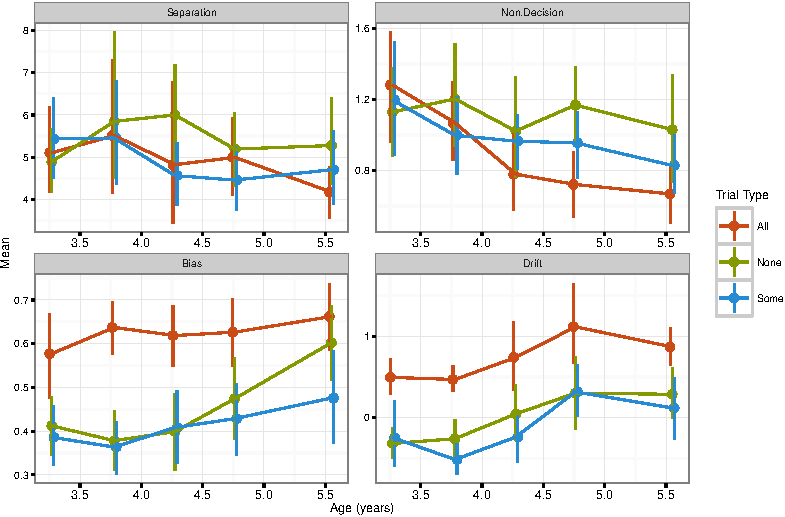
\includegraphics{figs/param_plot-1} 

}

\caption[Parameter estimates for drift diffusion model, split by accuracy and trial type]{Parameter estimates for drift diffusion model, split by accuracy and trial type. Error bars are 95 percent confidence intervals computed by nonparametric bootstrap.}\label{fig:param_plot}
\end{figure*}
\end{CodeChunk}

We again used mixed-effects models to predict DDM coefficients across
participants. As in the developmental DDM analysis, there were no
significant effects of separation or non-decision. And while drift rates
showed a significant effect of accuracy, because we estimated parameters
for high- and low-accuracy children separately, these differences are
expected.

In our bias estimates, however, we found a significant interaction
between accuracy group and trial type on ``some'' trials (\(\beta\) =
-0.18, \(p = .0013\)). This interaction suggests that bias (the starting
point in the diffusion process) might be an important factor in
successfully making a scalar implicature: More successful children were
less biased towards incorrect response alternatives, perhaps due to
greater knowledge about the quantifier scale.

\section{General Discussion}\label{general-discussion}

What makes scalar implicatures using quantifiers so hard for children?
The best current hypothesis posits that children do not have access to
the appropriate inferential alternatives and hence fail to consider them
in their pragmatic computation (Barner \& Bachrach, 2010; Barner et al.,
2011). But what are those alternatives? Recent work has suggested that
the negative alternative ``none'' may compete with ``some'' and ``all''
when making SIs. Although ``none'' is not typically considered an
alternative in Gricean theories (Grice, 1975; Horn, 1972), it
nevertheless provides a relevant lexical alternative along the
quantifier scale. Our findings here are consistent with this account and
provide some additional support. Using a new method, we replicated the
pattern found in previous studies that those children who succeed in
comprehending the quantifier ``none'' are also able to make SIs
(Horowitz \& Frank, 2015; Horowitz et al., in prep.). In addition, our
data revealed a speed-accuracy trade-off, such that reaction times in
those trials for which children succeeded in making SIs were slower
overall.

One interpretation of this speed-accuracy trade-off is that children who
have more inferential alternatives accessible to them (e.g.~are
considering ``none,'' ``some,'' and ``all'' together) are both better at
making SIs and slower to make them due to the processing cost of making
the inference. Our data are consistent with this account, which is also
supported by an exploratory drift diffusion model analysis. We fit a DDM
to our data for children who succeeded in making scalar implicatures
versus children who failed. The model suggested that bias in ``some''
and ``none'' trials might be a key factor related to success---that is,
children who were considering ``some'' and ``all'' responses equally in
their decision were more likely to make the SI. Both of these findings
are again consistent with the idea that weighing alternatives
appropriately in the SI computation is critical to success.

The speed-accuracy patterns we report are correlational, however, and
other accounts are consistent with these findings as well. For example,
some third factor (say inhibitory control) could underlie the ability to
succeed in ``some'' and ``none'' trials and also explain why some
children are able to inhibit their response long enough to complete the
SI computation. Horowitz et al. (in prep.) did not find evidence of
correlations between individuals' SI abilities and their executive
function using one popular measure (the dimensional change card sort).
Other versions of this account (or other accounts entirely) are still
possible, however, and should be explored in future work. Nevertheless,
our present work suggests that there is a meaningful relationship
between children's accuracy and processing times in making scalar
implicatures.

\section{Acknowledgements}\label{acknowledgements}

Thanks to Bing Nursery School and the San Jose Children's Discovery
Museum. Thanks also to Veronica Cristiano, Rachel Walker, and Tamara
Mekler for their help with data collection, and to Kara Weisman and Ann
Nordmeyer for their assistance creating stimuli. This work was supported
by NSF BCS 1456077.

\section{References}\label{references}

\setlength{\parindent}{-0.1in} \setlength{\leftskip}{0.125in} \noindent

Barner, D., \& Bachrach, A. (2010). Inference and exact numerical
representation in early language development. \emph{Cognitive
Psychology}, \emph{60}(1), 40--62.

Barner, D., Brooks, N., \& Bale, A. (2011). Accessing the unsaid: The
role of scalar alternatives in children’s pragmatic inference.
\emph{Cognition}, \emph{118}(1), 84--93.

Degen, J., \& Tanenhaus, M. K. (2015). Processing scalar implicature: A
constraint-based approach. \emph{Cognitive Science}, \emph{39}(4),
667--710.

Franke, M. (2014). Typical use of quantifiers: A probabilistic speaker
model. In \emph{Proceedings of the 36th annual conference of the
cognitive science society} (pp. 487--492).

Goodman, N. D., \& Stuhlmuller, A. (2013). Knowledge and implicature:
Modeling language understanding as social cognition. \emph{Topics in
Cognitive Science}, \emph{5}(1), 173--184.

Grice, H. P. (1975). Logic and conversation. In P. Cole \& J. Morgan
(Eds.), \emph{Syntax and semantics} (Vol. 3). New York: Academic Press.

Horn, L. R. (1972). \emph{On the semantic properties of logical
operators.} (PhD thesis). University of California, Los Angeles.

Horowitz, A., \& Frank, M. C. (2015). Sources of developmental change in
pragmatic inferences about scalar terms. In \emph{Proceedings of the
37th annual conference of the cognitive science society.}

Horowitz, A., Schneider, R. M., \& Frank, M. C. (in prep.). The trouble
with quantifiers: Exploring children's deficits in scalar implicatures.

Huang, Y. T., \& Snedeker, J. (2009). Online interpretation of scalar
quantifiers: Insight into the semantics-pragmatics interface.
\emph{Cognitive Psychology}, \emph{58}(3), 376--415.

Katsos, N., \& Bishop, D. (2011). Pragmatic tolerance: Implications for
the acquisition of informativeness and implicature. \emph{Cognition},
\emph{120}(1), 67--81.

Levinson, S. C. (2000). \emph{Presumptive meanings: The theory of
generalized conversational implicature}. MIT Press.

Noveck, I. (2001). When children are more logical than adults:
Experimental investigations of scalar implicature. \emph{Cognition},
\emph{78}(2), 165--188.

Papafragou, A., \& Musolino, J. (2003). Scalar implicatures: Experiments
at the semantics-pragmatics interface. \emph{Cognition}, \emph{86}(3),
253--282.

Ratcliff, R. (1978). A theory of memory retrieval. \emph{Psychological
Review}, \emph{85}(2), 59.

Ratcliff, R., \& Rouder, J. (1998). Modeling response times for
two-choice decisions. \emph{Psychologial Science}, \emph{9}(5),
347--356.

Skordos, D., \& Papafragou, A. (in press). Children's derivation of
scalar implicatures: Alternatives and relevance. \emph{Cognition}.

\end{document}
